% =============================================================================
% idea2/emi.tex — Perfil de Proyecto de Grado
% Estructura según: Guía de Elaboración de Perfil Trabajos de Grado
% Universidad Privada del Valle — DAAP, 1ra Ed. 2019
%
% Motor requerido: XeLaTeX
%   Compilar con: latexmk -xelatex emi.tex  (ejecutar desde esta carpeta)
% =============================================================================

\documentclass{univalle-perfil}

\usepackage{tikz}
\usetikzlibrary{shapes.geometric, arrows.meta, positioning, babel}
\usepackage{colortbl}

% Reiniciar la numeración de figuras y cuadros en cada sección (Figura 2.1, 6.1, ...)
\counterwithin{figure}{section}
\counterwithin{table}{section}

\graphicspath{{../}}
\addbibresource{perfil.bib}

% -----------------------------------------------------------------------------
% METADATOS DE LA CARÁTULA
% -----------------------------------------------------------------------------
\universidad{Universidad Privada del Valle}
\facultad{Facultad de Informática y Electrónica}
\carrera{Carrera de Licenciatura en Ingeniería de Sistemas}
\tituloTrabajo{Desarrollo de un módulo de inteligencia predictiva para el ERP ISI Mustang basado en el aprovechamiento de datos históricos operativos}
\modalidad{Proyecto de Grado}
\tituloOptar{Licenciatura en Ingeniería de Sistemas}
\postulante{Franco Javier Torrez Alvarado}
\tutor{Rolando Lara Sanchez}
\ciudad{Santa Cruz}
\pais{Bolivia}
\anio{2026}

% =============================================================================
\begin{document}

% --- Carátula ----------------------------------------------------------------
\makecaratula

% --- Índices -----------------------------------------------------------------
\pagenumbering{gobble}
\tableofcontents
\listoffigures
\listoftables

% --- Contenido principal -----------------------------------------------------
\pagenumbering{arabic}

% =============================================================================
% 1. INTRODUCCIÓN
% =============================================================================
\section{Introducción}

Los sistemas ERP constituyen el núcleo operativo de las empresas de ingeniería, registrando de forma continua datos de proyectos, certificaciones, recursos humanos, horas trabajadas, requisiciones y compras. Sin embargo, como señala \textcite{MLdrivenERP2023}, la mayoría de las organizaciones utilizan estos sistemas principalmente para la gestión operativa y la generación de reportes descriptivos, sin explotar el potencial predictivo que ofrecen los datos históricos acumulados. En el ámbito de la gestión de proyectos de ingeniería, el aprendizaje automático ha demostrado superar en precisión a los métodos tradicionales de planificación y control: \textcite{AIcostEstimation2024} demuestra, mediante una revisión sistemática de 39 estudios, que los modelos de inteligencia artificial mejoran significativamente la estimación de costos, mientras que \textcite{AutoMLpipeline2025} propone pipelines automatizados capaces de predecir costos y duración de proyectos con mayor exactitud que las herramientas convencionales basadas en el Earned Value Management.

ISI Mustang Bolivia, empresa con más de 25 años de operación en ingeniería y servicios tecnológicos para los sectores de gas y petróleo, energía y minería, se encuentra precisamente en esta situación. Su ERP acumula más de diez años de datos operativos que incluyen un activo de especial valor para el aprendizaje automático: registros históricos de desviaciones en certificaciones con sus causas documentadas, constituyendo un conjunto de datos etiquetados de aprendizaje supervisado que pocas organizaciones poseen. \textcite{XGBoostCostOverrun2026} demuestra que modelos como XGBoost alcanzan alta precisión en la predicción de sobrecostos en proyectos de construcción cuando se dispone de datos históricos estructurados, lo que respalda la viabilidad técnica de aprovechar el historial del ERP ISI Mustang para anticipar desviaciones y riesgos operativos.

El presente trabajo propone el desarrollo de un módulo de inteligencia predictiva integrado al ERP ISI Mustang que, mediante técnicas de aprendizaje automático aplicadas sobre datos históricos operativos, permita anticipar desviaciones y riesgos en la gestión de proyectos de ingeniería. El documento se organiza en las siguientes secciones: antecedentes del problema, objetivos, justificación, delimitación de la investigación, propuesta de solución, diseño metodológico, índice tentativo, marco teórico y cronograma.

% =============================================================================
% 2. ANTECEDENTES DEL PROBLEMA
% =============================================================================
\section{Antecedentes del Problema}

La aplicación de técnicas de inteligencia artificial sobre los datos generados por sistemas ERP ha sido objeto de creciente interés en la comunidad académica internacional. \textcite{MLdrivenERP2023} presenta una revisión comprensiva sobre el uso de aprendizaje automático para la optimización de sistemas ERP, identificando la predicción de desviaciones operativas y la mejora de la toma de decisiones como los casos de uso de mayor impacto. En el ámbito específico de la gestión de proyectos de ingeniería, \textcite{AIcostEstimation2024} sintetiza los resultados de 39 estudios publicados entre 2016 y 2024, concluyendo que los modelos de inteligencia artificial superan consistentemente a los métodos tradicionales en la estimación y predicción de costos.

En cuanto a trabajos específicos que abordan problemas análogos al planteado, \textcite{XGBoostCostOverrun2026} desarrolló un modelo de XGBoost explicable para predecir sobrecostos en proyectos de construcción a partir de datos históricos estructurados, superando en precisión a modelos tradicionales como la regresión lineal y los árboles de decisión simples; no obstante, su estudio se sustenta en conjuntos de datos del sector construcción y no contempla la integración del modelo en el sistema de información operativo de una empresa. Por su parte, \textcite{DomainAwareXGBoost2025} propuso un marco de XGBoost con restricciones de dominio para la predicción de retrasos en proyectos, alcanzando una precisión del 92\% y reduciendo el error de predicción de tiempo en aproximadamente un 80\% respecto a métodos convencionales como el Earned Value Management; sin embargo, su enfoque exige la definición manual de reglas de dominio y fue validado sobre un conjunto de datos acotado. Finalmente, \textcite{AutoMLpipeline2025} planteó un pipeline automatizado de aprendizaje automático para el pronóstico de costos y duración de proyectos, evidenciando que la integración de múltiples fuentes de datos mejora la precisión predictiva; aun así, dicho pipeline opera sobre datos consolidados de diversas organizaciones y no sobre el historial operativo de una empresa en particular.

Los antecedentes revisados confirman la viabilidad técnica de aplicar aprendizaje automático para anticipar desviaciones y riesgos en proyectos de ingeniería, pero comparten una limitación común: se desarrollan sobre conjuntos de datos públicos o multiorganizacionales y no se integran en el sistema de gestión operativo de la empresa que origina los datos. Adicionalmente, no se identificaron antecedentes de aplicación de inteligencia predictiva sobre los datos históricos del ERP ISI Mustang ni trabajos similares en el contexto de empresas de ingeniería bolivianas. Esta doble brecha —la ausencia de soluciones integradas al ERP y la falta de precedentes en el contexto local— constituye el punto de partida del presente proyecto de grado.

\subsection{Planteamiento del Problema}

ISI Mustang Bolivia gestiona proyectos integrales de tipo EPC en los sectores de gas, petróleo, minería y energía, apoyándose en un ERP propio que acumula más de diez años de datos históricos operativos. Sin embargo, dicha información se utiliza únicamente con fines descriptivos y de control inmediato, sin un mecanismo que permita identificar patrones o anticipar comportamientos futuros. Como consecuencia, la detección de desviaciones presupuestarias, retrasos y cuellos de botella ocurre de forma reactiva, limitando la capacidad de gestión proactiva de riesgos en proyectos de alta complejidad técnica y económica.

El diagrama de Ishikawa (Figura~\ref{fig:ishikawa}) sintetiza las principales causas que originan esta problemática, mientras que el análisis FODA (Cuadro~\ref{tab:foda}) resume la situación de la empresa frente a la explotación predictiva de sus datos.

\begin{figure}[htbp]
    \centering
    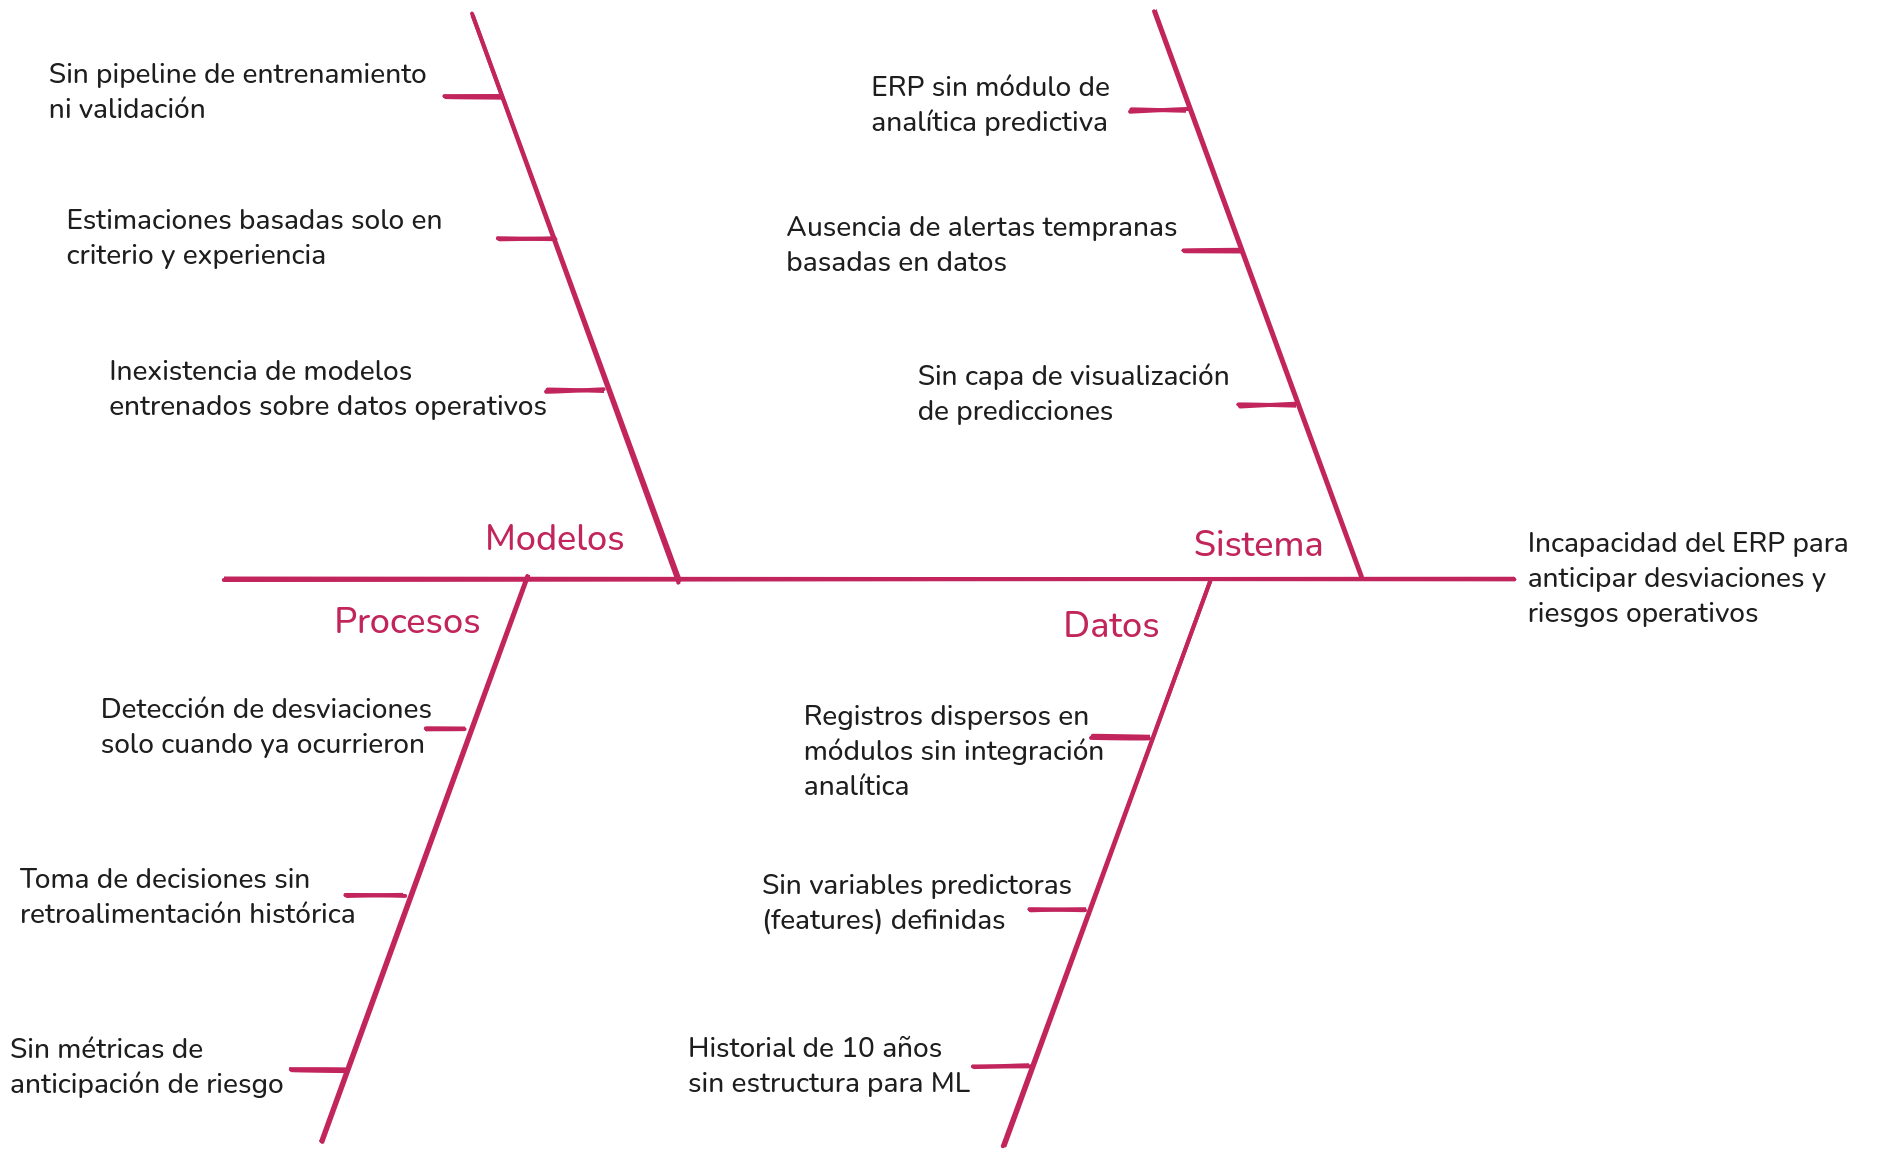
\includegraphics[width=\textwidth]{idea2/imagenes/ishikawa.png}
    \caption{Diagrama de Ishikawa — causas de la gestión reactiva de riesgos en proyectos EPC de ISI Mustang.}
    \label{fig:ishikawa}
\end{figure}

\begin{table}[htbp]
\centering
\small
\caption{Análisis FODA — ISI Mustang Bolivia respecto a la explotación predictiva de datos del ERP.}
\label{tab:foda}
\renewcommand{\arraystretch}{1.4}
\begin{tabular}{|p{0.46\textwidth}|p{0.46\textwidth}|}
\hline
\textbf{Fortalezas} & \textbf{Oportunidades} \\[2pt]
$\bullet$ Más de diez años de datos históricos operativos acumulados. \newline
$\bullet$ Registros de desviaciones con causas documentadas en el historial de proyectos. \newline
$\bullet$ Sistema de información propio con control total sobre los datos operativos.
&
$\bullet$ Alta demanda de gestión proactiva en proyectos de ingeniería del sector energético. \newline
$\bullet$ Creciente disponibilidad de soluciones de análisis predictivo en la industria. \newline
$\bullet$ Mejora del posicionamiento competitivo en la estimación y adjudicación de contratos. \\
\hline
\textbf{Debilidades} & \textbf{Amenazas} \\[2pt]
$\bullet$ Posibles inconsistencias en el registro histórico de información. \newline
$\bullet$ Ausencia de una cultura de análisis de datos en la organización. \newline
$\bullet$ Dependencia de la disciplina en el registro operativo para la calidad de los resultados.
&
$\bullet$ Resistencia al cambio por parte de los usuarios ante nuevas herramientas de gestión. \newline
$\bullet$ Cambios en los procesos operativos pueden reducir la vigencia de los modelos desarrollados. \newline
$\bullet$ Baja adopción si los resultados no se comunican de forma clara a los usuarios clave. \\
\hline
\end{tabular}
\end{table}

\subsubsection{Formulación del Problema}

¿En qué medida un módulo de inteligencia predictiva basado en los datos históricos del ERP ISI Mustang permite anticipar desviaciones y riesgos en la gestión de proyectos de ingeniería EPC de la empresa?

\subsection{Árbol del Problema}

El árbol del problema (Figura~\ref{fig:arbol}) sintetiza las causas que originan la situación descrita y los efectos que de ella se derivan, complementando el análisis de causas presentado en el diagrama de Ishikawa.

\begin{figure}[htbp]
\centering
\resizebox{\textwidth}{!}{%
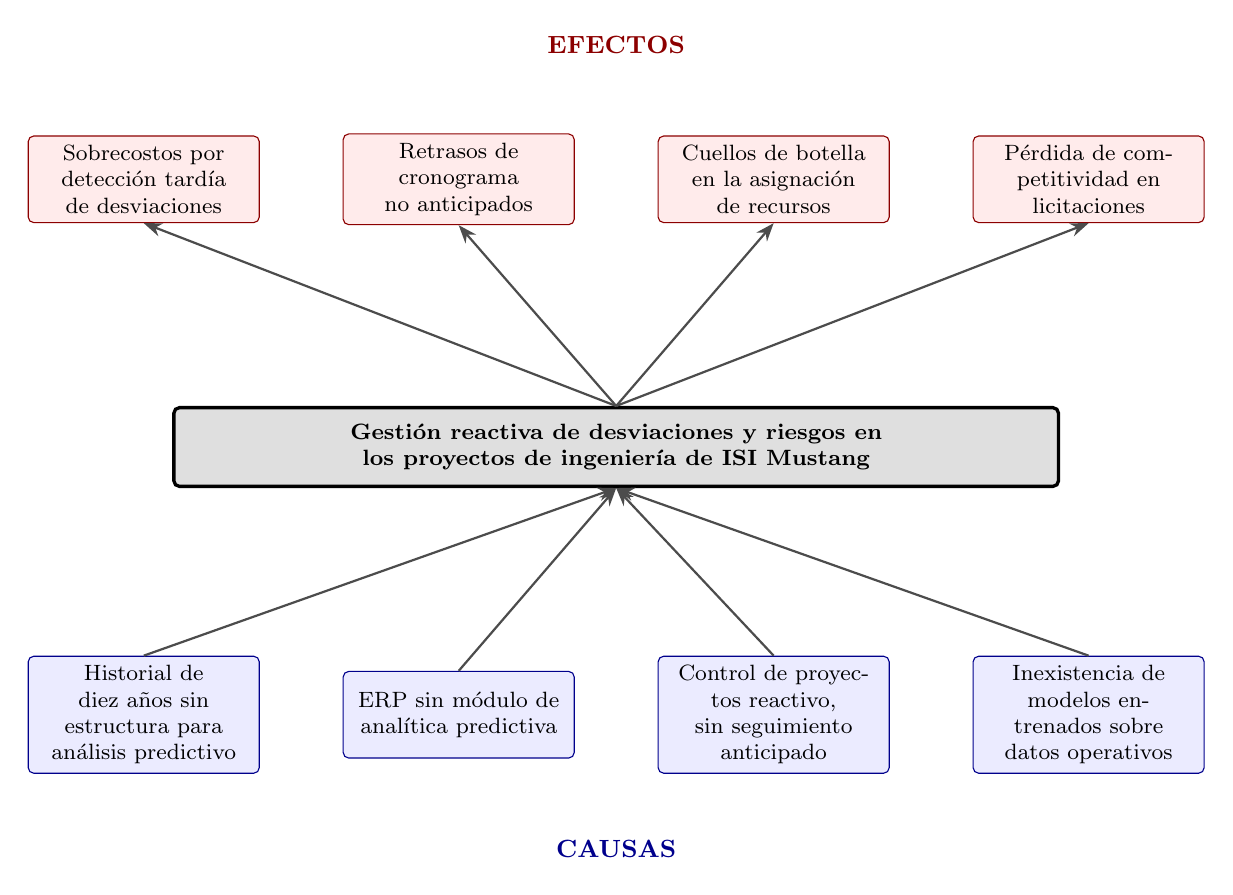
\begin{tikzpicture}[
    efecto/.style   = {rectangle, rounded corners=2pt, draw=red!55!black, fill=red!8,
                       text width=2.7cm, align=center, minimum height=1.1cm, font=\footnotesize},
    problema/.style = {rectangle, rounded corners=2pt, draw=black, fill=gray!25, very thick,
                       text width=11cm, align=center, minimum height=1cm, font=\footnotesize\bfseries},
    causa/.style    = {rectangle, rounded corners=2pt, draw=blue!55!black, fill=blue!8,
                       text width=2.7cm, align=center, minimum height=1.1cm, font=\footnotesize},
    banda/.style    = {font=\small\bfseries},
    arrow/.style    = {-{Stealth}, thick, gray!60!black},
]

% Problema central
\node[problema] (p) at (0,0) {Gestión reactiva de desviaciones y riesgos en los proyectos de ingeniería de ISI Mustang};

% Efectos
\node[efecto] (e1) at (-6,3.4) {Sobrecostos por detección tardía de desviaciones};
\node[efecto] (e2) at (-2,3.4) {Retrasos de cronograma no anticipados};
\node[efecto] (e3) at (2,3.4)  {Cuellos de botella en la asignación de recursos};
\node[efecto] (e4) at (6,3.4)  {Pérdida de competitividad en licitaciones};

% Causas
\node[causa] (c1) at (-6,-3.4) {Historial de diez años sin estructura para análisis predictivo};
\node[causa] (c2) at (-2,-3.4) {ERP sin módulo de analítica predictiva};
\node[causa] (c3) at (2,-3.4)  {Control de proyectos reactivo, sin seguimiento anticipado};
\node[causa] (c4) at (6,-3.4)  {Inexistencia de modelos entrenados sobre datos operativos};

% Bandas
\node[banda, text=red!55!black]  at (0,5.1)  {EFECTOS};
\node[banda, text=blue!55!black] at (0,-5.1) {CAUSAS};

% Flechas causas -> problema central
\draw[arrow] (c1.north) -- (p.south);
\draw[arrow] (c2.north) -- (p.south);
\draw[arrow] (c3.north) -- (p.south);
\draw[arrow] (c4.north) -- (p.south);

% Flechas problema central -> efectos
\draw[arrow] (p.north) -- (e1.south);
\draw[arrow] (p.north) -- (e2.south);
\draw[arrow] (p.north) -- (e3.south);
\draw[arrow] (p.north) -- (e4.south);

\end{tikzpicture}
}
\caption{Árbol del problema — causas y efectos de la gestión reactiva de desviaciones y riesgos en los proyectos de ISI Mustang.}
\label{fig:arbol}
\end{figure}

\subsection{Objeto de Estudio}

El proceso de gestión y control de desviaciones y riesgos en los proyectos de ingeniería de ISI Mustang, a partir de los datos históricos registrados en su ERP.

% =============================================================================
% 3. OBJETIVOS
% =============================================================================
\section{Objetivos}

\subsection{Objetivo General}

Desarrollar un módulo de inteligencia predictiva integrado al ERP ISI Mustang, mediante técnicas de aprendizaje automático aplicadas sobre datos históricos operativos, para anticipar desviaciones y riesgos en la gestión de proyectos de ingeniería EPC.

\subsection{Objetivos Específicos}

\begin{itemize}
    \item Analizar los datos históricos disponibles en los módulos del ERP ISI Mustang para identificar patrones de desviación y definir los casos de uso del módulo predictivo.
    \item Diseñar la arquitectura del módulo predictivo y seleccionar los modelos de aprendizaje automático adecuados para cada caso de uso identificado.
    \item Construir el pipeline de datos y entrenar los modelos predictivos para los casos de uso definidos.
    \item Integrar el módulo predictivo y su dashboard de visualización al ERP ISI Mustang.
    \item Evaluar la precisión de los modelos y la funcionalidad del módulo mediante métricas de rendimiento y pruebas con usuarios clave de ISI Mustang.
\end{itemize}

% =============================================================================
% 4. JUSTIFICACIÓN
% =============================================================================
\section{Justificación}

\subsection{Justificación Técnica}

El ERP de ISI Mustang acumula más de diez años de datos operativos distribuidos en múltiples módulos, constituyendo un volumen suficiente para el entrenamiento de modelos de aprendizaje automático. En particular, el módulo de certificaciones contiene registros históricos de desviaciones con sus causas documentadas, conformando un conjunto de datos etiquetados para aprendizaje supervisado que pocas organizaciones poseen. Las técnicas actuales de aprendizaje automático supervisado, en particular los modelos de gradient boosting, son suficientemente maduras para ser aplicadas sobre este tipo de datos tabulares operativos. Además, la integración de un módulo predictivo al ERP existente es técnicamente viable mediante acceso directo a la base de datos del sistema.

\subsection{Justificación Económica}

Los proyectos de tipo EPC que ejecuta ISI Mustang en sectores como gas y petróleo, minería y energía involucran presupuestos de alta envergadura, donde la detección temprana de desviaciones puede reducir significativamente los costos de corrección. La anticipación de cuellos de botella en la asignación de recursos permite evitar sobrecostos por sobreasignación o tiempos improductivos. Asimismo, la capacidad predictiva sobre propuestas y proyectos mejora la competitividad de la empresa en la estimación y adjudicación de nuevos contratos.

\subsection{Justificación Social}

Una gestión de proyectos más proactiva y basada en datos garantiza entregas más confiables en sectores críticos para el desarrollo de Bolivia, como los hidrocarburos, la energía y la minería. La reducción de la gestión reactiva disminuye la carga operativa de los equipos de proyecto, contribuyendo a mejores condiciones de trabajo. A nivel más amplio, el proyecto demuestra que empresas bolivianas pueden capitalizar sus propios datos históricos mediante inteligencia artificial, aportando al desarrollo tecnológico nacional.

% =============================================================================
% 5. DELIMITACIÓN DE LA INVESTIGACIÓN
% =============================================================================
\section{Delimitación de la Investigación}

\subsection{Temática}

El presente trabajo se delimita a las áreas de aprendizaje automático supervisado, ingeniería de datos y analítica predictiva, aplicadas sobre los datos operativos del ERP ISI Mustang. En cuanto a la gestión de proyectos, el estudio se circunscribe a proyectos de tipo EPC ejecutados por ISI Mustang. Quedan fuera del alcance las fuentes de datos externas al ERP, como sensores IoT, datos de mercado o información climática, así como los módulos del sistema que no se encuentren activos o poblados con datos históricos suficientes.

\subsection{Espacial}

El estudio se desarrolla en las instalaciones de ISI Mustang Bolivia, con sede en Santa Cruz de la Sierra, Bolivia. Los datos históricos utilizados corresponden a proyectos ejecutados por la empresa principalmente en territorio boliviano. El módulo de inteligencia predictiva desarrollado será integrado y validado en el ERP operativo de ISI Mustang en su sede central.

\subsection{Temporal}

Los datos históricos utilizados para el entrenamiento de los modelos de aprendizaje automático abarcan un período de más de diez años de operación del ERP ISI Mustang. El desarrollo del proyecto de grado se estima entre abril y agosto de 2026, período que comprende las etapas de análisis, diseño, construcción y evaluación del módulo predictivo.

En cuanto a la validez temporal de la investigación, dado que los modelos predictivos se entrenan sobre patrones históricos, se estima que la solución mantiene su vigencia mientras las condiciones operativas de la empresa permanezcan estables. Se recomienda un reentrenamiento periódico de los modelos —de forma anual o ante cambios sustanciales en los procesos de la empresa— con el fin de mitigar la pérdida de precisión por deriva de datos (\textit{model drift}).

% =============================================================================
% 6. PROPUESTA DE SOLUCIÓN AL PLANTEAMIENTO DEL PROBLEMA
% =============================================================================
\section{Propuesta de Solución al Planteamiento del Problema}

Se propone el desarrollo de un módulo de inteligencia predictiva organizado como una arquitectura por capas, que abarca desde las fuentes de datos del ERP hasta la presentación de las predicciones al usuario. La solución se integra al ERP existente de ISI Mustang sin modificar su arquitectura central: el módulo predictivo opera como un componente independiente que consume los datos históricos del sistema y expone sus resultados a través de un microservicio. La Figura~\ref{fig:arquitectura} presenta esta arquitectura, diferenciando los componentes nuevos del módulo predictivo de los componentes ya existentes del ERP.

\begin{figure}[H]
\centering
\resizebox{\textwidth}{!}{%
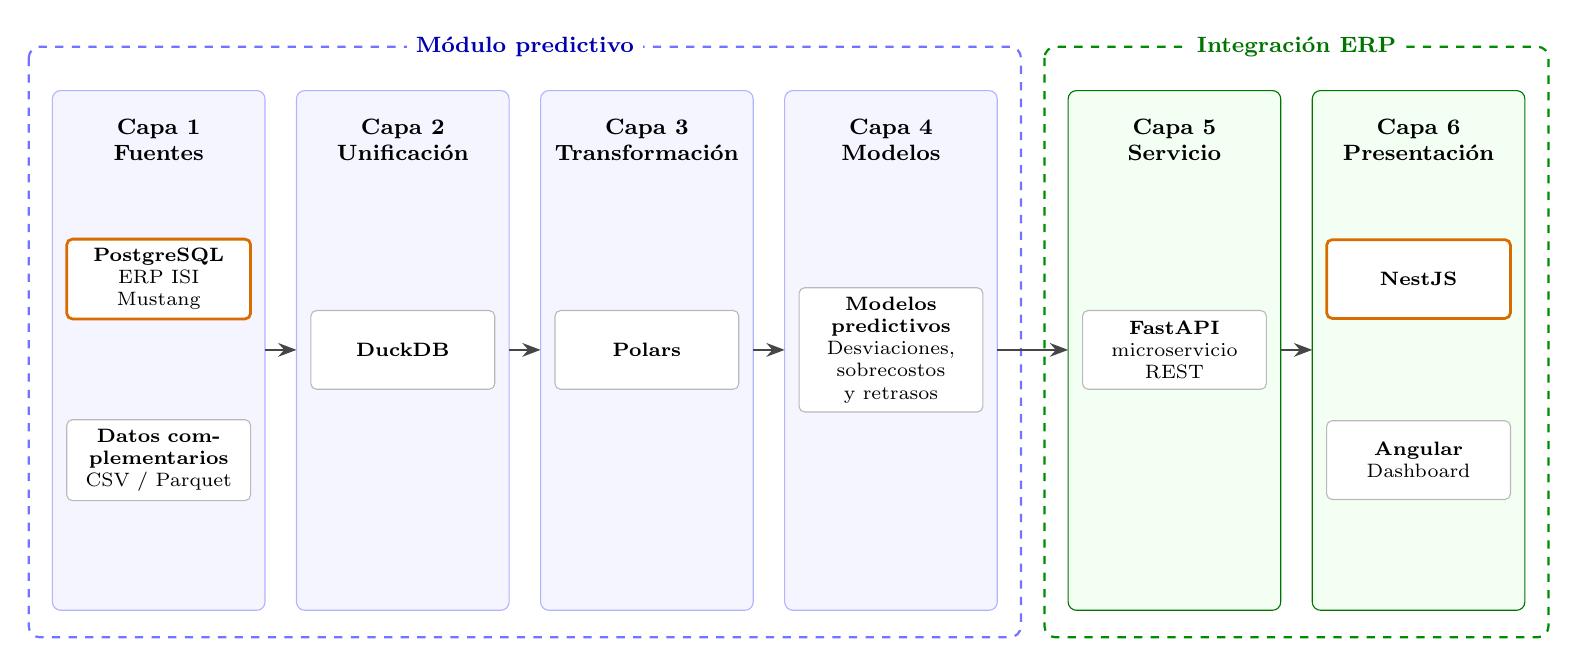
\begin{tikzpicture}[
    grupoP/.style = {draw=blue!55, dashed, thick, rounded corners=4pt},
    grupoE/.style = {draw=green!55!black, dashed, thick, rounded corners=4pt},
    capaP/.style  = {draw=blue!30, fill=blue!4, rounded corners=3pt},
    capaE/.style  = {draw=green!45!black, fill=green!5, rounded corners=3pt},
    comp/.style   = {draw=gray!55, fill=white, rounded corners=2pt, align=center,
                     text width=2.1cm, minimum height=1cm, font=\scriptsize},
    compex/.style = {draw=orange!85!black, line width=1pt, fill=white, rounded corners=2pt,
                     align=center, text width=2.1cm, minimum height=1cm, font=\scriptsize},
    titulo/.style = {align=center, font=\footnotesize\bfseries, anchor=north},
    arr/.style    = {-{Stealth}, thick, gray!55!black},
]

% --- Contenedores de grupo (dashed) ---
\draw[grupoP] (-1.65,0.55) rectangle (10.95,-6.95);
\draw[grupoE] (11.25,0.55) rectangle (17.65,-6.95);
\node[fill=white, text=blue!70!black, font=\footnotesize\bfseries] at (4.65,0.55) {Módulo predictivo};
\node[fill=white, text=green!45!black, font=\footnotesize\bfseries] at (14.45,0.55) {Integración ERP};

% --- Contenedores de capa ---
\node[capaP, minimum width=2.7cm, minimum height=6.6cm, anchor=north] at (0,0) {};
\node[capaP, minimum width=2.7cm, minimum height=6.6cm, anchor=north] at (3.1,0) {};
\node[capaP, minimum width=2.7cm, minimum height=6.6cm, anchor=north] at (6.2,0) {};
\node[capaP, minimum width=2.7cm, minimum height=6.6cm, anchor=north] at (9.3,0) {};
\node[capaE, minimum width=2.7cm, minimum height=6.6cm, anchor=north] at (12.9,0) {};
\node[capaE, minimum width=2.7cm, minimum height=6.6cm, anchor=north] at (16.0,0) {};

% --- Títulos de capa ---
\node[titulo] at (0,-0.25)    {Capa 1\\Fuentes};
\node[titulo] at (3.1,-0.25)  {Capa 2\\Unificación};
\node[titulo] at (6.2,-0.25)  {Capa 3\\Transformación};
\node[titulo] at (9.3,-0.25)  {Capa 4\\Modelos};
\node[titulo] at (12.9,-0.25) {Capa 5\\Servicio};
\node[titulo] at (16.0,-0.25) {Capa 6\\Presentación};

% --- Componentes ---
\node[compex] at (0,-2.4)   {\textbf{PostgreSQL}\\ERP ISI Mustang};
\node[comp]   at (0,-4.7)   {\textbf{Datos complementarios}\\CSV / Parquet};
\node[comp]   at (3.1,-3.3) {\textbf{DuckDB}};
\node[comp]   at (6.2,-3.3) {\textbf{Polars}};
\node[comp]   at (9.3,-3.3) {\textbf{Modelos predictivos}\\Desviaciones, sobrecostos y retrasos};
\node[comp]   at (12.9,-3.3){\textbf{FastAPI}\\microservicio REST};
\node[compex] at (16.0,-2.4){\textbf{NestJS}};
\node[comp]   at (16.0,-4.7){\textbf{Angular}\\Dashboard};

% --- Flechas entre capas ---
\draw[arr] (1.35,-3.3)  -- (1.75,-3.3);
\draw[arr] (4.45,-3.3)  -- (4.85,-3.3);
\draw[arr] (7.55,-3.3)  -- (7.95,-3.3);
\draw[arr] (10.65,-3.3) -- (11.55,-3.3);
\draw[arr] (14.25,-3.3) -- (14.65,-3.3);

\end{tikzpicture}
}
\caption{Arquitectura por capas del módulo predictivo y su integración con el ERP ISI Mustang.}
\label{fig:arquitectura}
\end{figure}

La capa de fuentes reúne los datos operativos del ERP (PostgreSQL) junto con datos complementarios en archivos (CSV/Parquet); la capa de unificación los consolida mediante DuckDB; la capa de transformación realiza la ingeniería de variables con Polars; y la capa de modelos entrena los modelos predictivos para los casos de uso definidos. Posteriormente, la capa de servicio expone los modelos como una API REST con FastAPI, que el backend NestJS del ERP consume para presentar las predicciones en un dashboard de Angular.

El siguiente diagrama de flujo (Figura~\ref{fig:flujo}) describe el proceso predictivo de extremo a extremo, desde los datos históricos hasta la visualización del resultado por el usuario.

\begin{figure}[H]
\centering
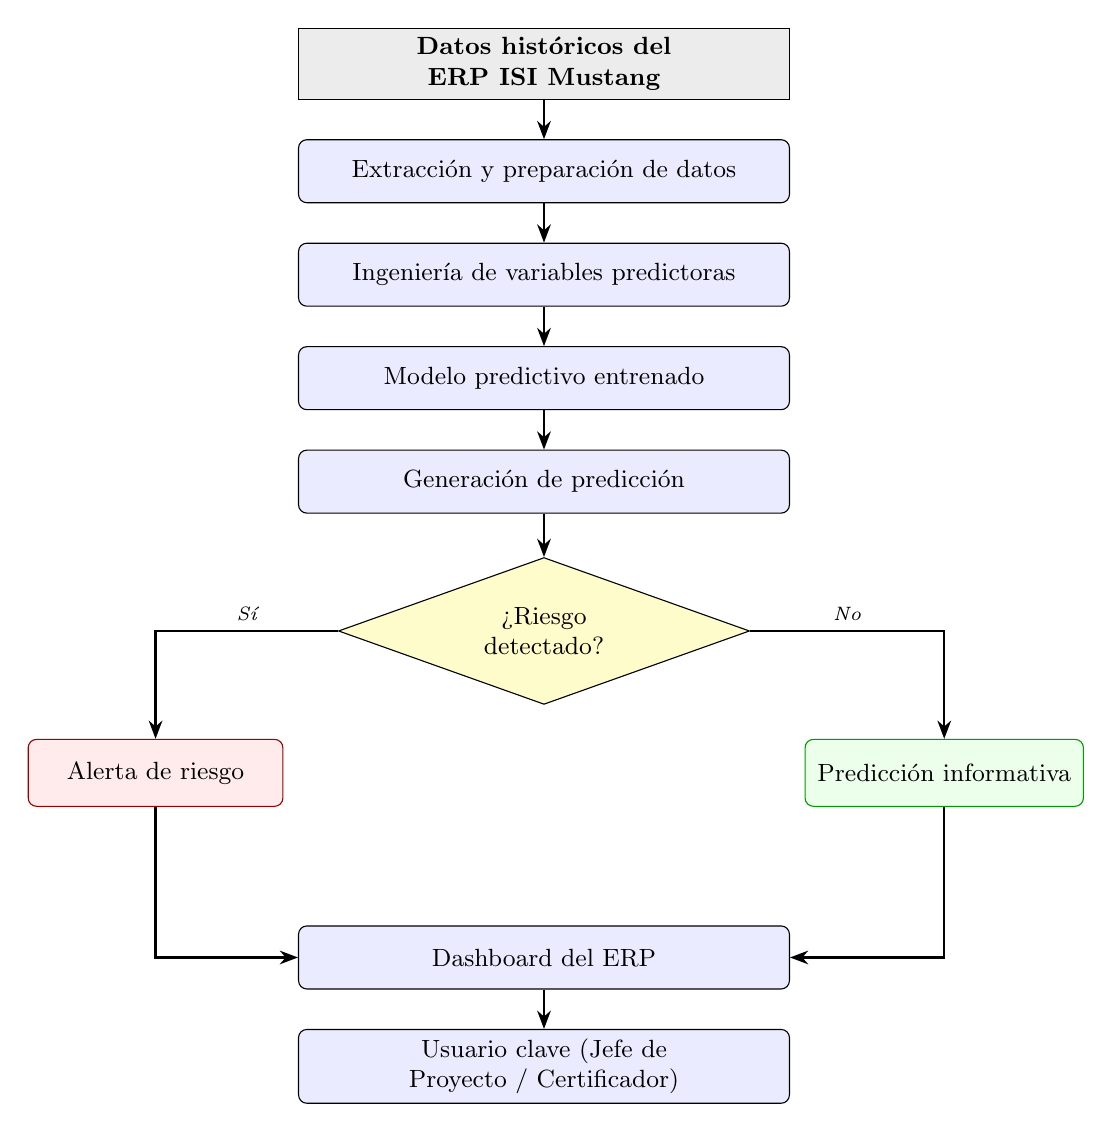
\begin{tikzpicture}[
    node distance = 0.5cm,
    box/.style      = {rectangle, rounded corners=3pt, draw, fill=blue!8,
                       text width=6cm, align=center, minimum height=0.8cm, font=\small},
    dbbox/.style    = {rectangle, draw, fill=gray!15, text width=6cm,
                       align=center, minimum height=0.85cm, font=\small\bfseries},
    decision/.style = {diamond, draw, fill=yellow!20, text width=3cm,
                       align=center, font=\small, aspect=2.8, inner sep=2pt},
    alert/.style    = {rectangle, rounded corners=3pt, draw=red!60!black, fill=red!8,
                       text width=3cm, align=center, minimum height=0.85cm, font=\small},
    info/.style     = {rectangle, rounded corners=3pt, draw=green!60!black, fill=green!8,
                       text width=3.3cm, align=center, minimum height=0.85cm, font=\small},
    arrow/.style    = {->, >=Stealth, thick},
]

\node[dbbox]                             (erp)    {Datos históricos del ERP ISI Mustang};
\node[box,     below=of erp]             (extr)   {Extracción y preparación de datos};
\node[box,     below=of extr]            (ing)    {Ingeniería de variables predictoras};
\node[box,     below=of ing]             (modelo) {Modelo predictivo entrenado};
\node[box,     below=of modelo]          (pred)   {Generación de predicción};
\node[decision, below=0.55cm of pred]    (dec)    {¿Riesgo\\detectado?};
\node[alert, below left=0.9cm and 2.0cm of dec]  (alerta) {Alerta de riesgo};
\node[info,  below right=0.9cm and 2.0cm of dec] (normal) {Predicción informativa};
\node[box,     below=2.8cm of dec]       (dash)   {Dashboard del ERP};
\node[box,     below=of dash]            (user)   {Usuario clave (Jefe de Proyecto / Certificador)};

\draw[arrow] (erp)    -- (extr);
\draw[arrow] (extr)   -- (ing);
\draw[arrow] (ing)    -- (modelo);
\draw[arrow] (modelo) -- (pred);
\draw[arrow] (pred)   -- (dec);
\draw[arrow] (dec) -| node[near start, above, font=\scriptsize\itshape] {Sí} (alerta);
\draw[arrow] (dec) -| node[near start, above, font=\scriptsize\itshape] {No} (normal);
\draw[arrow] (alerta) |- (dash);
\draw[arrow] (normal) |- (dash);
\draw[arrow] (dash)   -- (user);

\end{tikzpicture}
\caption{Diagrama de flujo del proceso predictivo — desde los datos históricos del ERP hasta la visualización del resultado por el usuario.}
\label{fig:flujo}
\end{figure}

% =============================================================================
% 7. DISEÑO METODOLÓGICO
% =============================================================================
\section{Diseño Metodológico}

\subsection{Tipo de Investigación}

El presente trabajo corresponde a una investigación aplicada, dado que utiliza conocimiento científico existente en el área del aprendizaje automático para dar solución a un problema concreto en el contexto operativo de ISI Mustang Bolivia. De acuerdo con sus fases, combina tres niveles de alcance: exploratorio, en la etapa inicial de comprensión y caracterización de los datos históricos del ERP; descriptivo, para identificar y caracterizar las variables operativas relevantes y los patrones de desviación; y correlacional, al modelar las relaciones entre dichas variables —como horas trabajadas, líneas de presupuesto y certificaciones— con el fin de anticipar desviaciones y riesgos en proyectos de ingeniería.

\subsection{Método de Investigación}

El presente trabajo adopta un enfoque mixto, dado que combina la recolección y el análisis de datos cuantitativos —los registros históricos almacenados en el ERP— con datos cualitativos provenientes de las entrevistas a usuarios clave. Para operacionalizar este enfoque se emplean los siguientes métodos:

Análisis documental: se utilizará para la revisión de literatura científica sobre aprendizaje automático, analítica predictiva y sistemas ERP, con el fin de establecer los fundamentos teóricos del trabajo.

Histórico-lógico: se aplicará sobre los datos históricos acumulados en el ERP durante más de diez años de operación, permitiendo identificar patrones y tendencias en el comportamiento de los proyectos a lo largo del tiempo.

Modelación: se empleará para la construcción de modelos matemáticos de aprendizaje automático que representen el comportamiento de las variables operativas y permitan generar predicciones.

Enfoque de sistemas: se utilizará para analizar el ERP ISI Mustang como un sistema con entradas, procesos y salidas, identificando las interrelaciones entre sus módulos y los flujos de datos relevantes para el módulo predictivo.

\subsection{Técnicas e Instrumentos de Investigación}

\subsubsection{Técnicas}

Análisis de datos: se aplicará sobre los registros históricos almacenados en el ERP ISI Mustang, con el propósito de identificar variables predictoras, detectar patrones de comportamiento y construir los conjuntos de datos necesarios para el entrenamiento de los modelos de aprendizaje automático.

Entrevista: se aplicará a usuarios clave del ERP en ISI Mustang Bolivia, con el fin de relevar requisitos funcionales del módulo predictivo, validar las predicciones generadas y recoger criterios de utilidad desde la perspectiva operativa.

Pruebas de los modelos predictivos: se aplicarán sobre un conjunto de datos de prueba independiente para evaluar el desempeño de los modelos entrenados. Para los casos de clasificación se emplearán indicadores como la exactitud, la precisión, la sensibilidad, el F1-score y la matriz de confusión; para los casos de regresión se utilizarán el error cuadrático medio (RMSE), el error absoluto medio (MAE) y el coeficiente de determinación (R\textsuperscript{2}). Adicionalmente, se aplicará validación cruzada para verificar la estabilidad de los resultados.

\subsubsection{Instrumentos}

Para el análisis de datos: scripts de extracción y transformación de datos, y cuadernos de análisis exploratorio (notebooks).

Para la entrevista: guía de entrevista semiestructurada dirigida a usuarios clave del sistema.

Para las pruebas de los modelos: cuadro de métricas de evaluación y rutinas de validación cruzada.

\subsection{Población y Muestra}

Análisis de datos: la población corresponde a la totalidad de registros históricos generados en el ERP ISI Mustang durante su período operativo. Se trabajará con el conjunto completo de datos disponibles en los módulos relevantes para los casos de predicción definidos.

Entrevista: la población está conformada por aproximadamente 20 usuarios del ERP en ISI Mustang Bolivia. La muestra será de 5 a 8 usuarios clave seleccionados mediante muestreo no probabilístico intencional, priorizando perfiles con roles de jefe de proyecto, certificador y administrador del sistema.

% =============================================================================
% 8. ÍNDICE TENTATIVO
% =============================================================================
\section{Índice Tentativo}

\begin{indicetentativo}
INTRODUCCIÓN \\[2pt]
CAPÍTULO I. MARCO GENERAL \\
\quad 1.1 Antecedentes \\
\quad 1.2 Planteamiento del Problema \\
\quad\quad 1.2.1 Formulación del Problema \\
\quad 1.3 Objetivos \\
\quad\quad 1.3.1 Objetivo General \\
\quad\quad 1.3.2 Objetivos Específicos \\
\quad 1.4 Justificación \\
\quad\quad 1.4.1 Justificación Técnica \\
\quad\quad 1.4.2 Justificación Económica \\
\quad\quad 1.4.3 Justificación Social \\
\quad 1.5 Metodología \\
\quad\quad 1.5.1 Tipo de Investigación \\
\quad\quad 1.5.2 Método de Investigación \\
\quad\quad 1.5.3 Técnicas e Instrumentos de Investigación \\
\quad\quad 1.5.4 Población y Muestra \\[2pt]
CAPÍTULO II. MARCO TEÓRICO Y TECNOLÓGICO \\
\quad 2.1 Sistemas ERP \\
\quad\quad 2.1.1 Definición y Características \\
\quad\quad 2.1.2 ERP en Empresas de Ingeniería \\
\quad\quad 2.1.3 ERP en el Sector de Petróleo, Gas y Minería \\
\quad 2.2 Aprendizaje Automático \\
\quad\quad 2.2.1 Tipos de Aprendizaje \\
\quad\quad 2.2.2 Aprendizaje Supervisado \\
\quad\quad 2.2.3 Algoritmos de Aprendizaje Supervisado: Gradient Boosting y XGBoost \\
\quad\quad 2.2.4 Feature Engineering \\
\quad 2.3 Analítica Predictiva \\
\quad\quad 2.3.1 Definición y Aplicaciones \\
\quad\quad 2.3.2 Analítica Predictiva en Gestión de Proyectos \\
\quad\quad 2.3.3 Predicción de Desviaciones y Costos \\
\quad 2.4 Gestión de Proyectos EPC \\
\quad\quad 2.4.1 Definición y Características \\
\quad\quad 2.4.2 Certificaciones y Control de Avance \\
\quad\quad 2.4.3 Desviaciones Presupuestarias y de Cronograma \\
\quad 2.5 Ingeniería de Software \\
\quad\quad 2.5.1 Proceso de Desarrollo de Software \\
\quad\quad 2.5.2 Metodología de Desarrollo Iterativa e Incremental \\
\quad\quad 2.5.3 Arquitectura de Software por Capas \\
\quad 2.6 Tecnologías del Stack de Desarrollo \\
\quad\quad 2.6.1 Python y su Ecosistema ML \\
\quad\quad 2.6.2 DuckDB y Polars \\
\quad\quad 2.6.3 FastAPI como Microservicio \\
\quad\quad 2.6.4 NestJS y Angular \\[2pt]
CAPÍTULO III. ANÁLISIS Y DISEÑO DEL SISTEMA PROPUESTO \\
\quad 3.1 Análisis de Datos Históricos del ERP \\
\quad\quad 3.1.1 Exploración y Caracterización de Datos \\
\quad\quad 3.1.2 Identificación de Variables Predictoras \\
\quad\quad 3.1.3 Definición de Casos de Uso Predictivos \\
\quad 3.2 Requerimientos del Sistema \\
\quad\quad 3.2.1 Requerimientos Funcionales \\
\quad\quad 3.2.2 Requerimientos No Funcionales \\
\quad 3.3 Diseño de la Arquitectura del Módulo Predictivo \\
\quad\quad 3.3.1 Arquitectura por Capas \\
\quad\quad 3.3.2 Diseño del Pipeline de Datos \\
\quad\quad 3.3.3 Diseño de Modelos ML \\
\quad\quad 3.3.4 Diseño de la API Predictiva \\
\quad\quad 3.3.5 Diseño del Dashboard \\[2pt]
CAPÍTULO IV. CONSTRUCCIÓN E IMPLEMENTACIÓN DEL SISTEMA \\
\quad 4.1 Pipeline de Extracción y Transformación de Datos \\
\quad\quad 4.1.1 Integración DuckDB con PostgreSQL \\
\quad\quad 4.1.2 Transformación de Datos con Polars \\
\quad\quad 4.1.3 Feature Engineering \\
\quad 4.2 Entrenamiento de Modelos Predictivos \\
\quad\quad 4.2.1 Modelo de Desviación en Certificaciones \\
\quad\quad 4.2.2 Modelo de Sobrecosto de Proyectos \\
\quad\quad 4.2.3 Modelo de Retraso en Cronograma \\
\quad 4.3 Desarrollo del Microservicio FastAPI \\
\quad 4.4 Integración con el ERP \\
\quad\quad 4.4.1 Endpoints de Predicción en NestJS \\
\quad\quad 4.4.2 Dashboard de Inteligencia Predictiva en Angular \\
\quad 4.5 Evaluación y Validación \\
\quad\quad 4.5.1 Métricas de Rendimiento de Modelos \\
\quad\quad 4.5.2 Pruebas con Usuarios Clave \\[2pt]
CONCLUSIONES \\
RECOMENDACIONES \\
REFERENCIAS BIBLIOGRÁFICAS \\
ANEXOS
\end{indicetentativo}

% =============================================================================
% 9. MARCO TEÓRICO
% =============================================================================
\section{Marco Teórico}

Los fundamentos teóricos del presente trabajo se organizan en seis áreas del conocimiento: sistemas ERP, aprendizaje automático, analítica predictiva, gestión de proyectos EPC, ingeniería de software y tecnologías del stack de desarrollo. Cada área aporta los conceptos necesarios para comprender el problema, justificar el enfoque metodológico y sustentar las decisiones técnicas del módulo propuesto.

\subsection{Sistemas ERP}

Los sistemas de planificación de recursos empresariales (ERP, por sus siglas en inglés Enterprise Resource Planning) son plataformas de software integradas que centralizan y gestionan los procesos operativos de una organización en un único sistema de información. Un ERP reúne datos de múltiples áreas funcionales —como finanzas, recursos humanos, compras, producción y gestión de proyectos— en una base de datos compartida, eliminando la fragmentación de la información y proporcionando una visión unificada de las operaciones \parencite{MLdrivenERP2023}.

En el contexto de empresas de ingeniería, los sistemas ERP adquieren una dimensión especial dado que deben gestionar proyectos de alta complejidad técnica y económica, con múltiples etapas, equipos multidisciplinarios y presupuestos considerables. \textcite{Rashid2019} destaca que la implementación de ERP en el sector de petróleo y gas presenta desafíos específicos relacionados con la trazabilidad de costos por proyecto, la gestión de recursos en campo y el control de certificaciones periódicas.

A pesar de que los sistemas ERP generan volúmenes significativos de datos operativos a lo largo de su ciclo de vida, la explotación analítica de dichos datos ha sido históricamente limitada. \textcite{MLdrivenERP2023} señala que la mayoría de las organizaciones utilizan sus ERP principalmente para la gestión operativa y la generación de reportes descriptivos, sin aprovechar el potencial predictivo que ofrecen los datos históricos acumulados. Este escenario representa una oportunidad para la aplicación de técnicas de aprendizaje automático sobre los datos del ERP, con el fin de transformar la información histórica en capacidad predictiva.

\subsection{Aprendizaje Automático}

El aprendizaje automático (machine learning) es una rama de la inteligencia artificial que desarrolla algoritmos capaces de aprender patrones a partir de datos y realizar predicciones sin ser explícitamente programados para cada tarea. A diferencia de los sistemas basados en reglas, los modelos de aprendizaje automático mejoran su rendimiento a medida que disponen de mayor cantidad de datos de entrenamiento.

El aprendizaje supervisado es el paradigma más relevante para el presente trabajo. En este enfoque, el modelo se entrena con un conjunto de datos etiquetados, es decir, datos para los cuales se conoce el resultado esperado. A partir de estos ejemplos, el modelo aprende la relación entre las variables de entrada (features) y la variable objetivo, con el fin de generalizar dicha relación a nuevos datos. Dentro del aprendizaje supervisado se distinguen dos tipos de tareas: la clasificación, cuyo objetivo es predecir una categoría discreta, y la regresión, cuyo objetivo es predecir un valor continuo. Para el módulo predictivo propuesto, ambos tipos son aplicables: clasificación para determinar si un proyecto presentará desviación, y regresión para estimar la magnitud de dicha desviación.

Entre los algoritmos de aprendizaje supervisado más utilizados en la predicción de resultados en proyectos de ingeniería destaca el gradient boosting, y en particular XGBoost (Extreme Gradient Boosting). \textcite{XGBoostCostOverrun2026} demuestra que los modelos XGBoost ofrecen alta precisión en la predicción de sobrecostos en proyectos de construcción, superando a modelos tradicionales como la regresión lineal y los árboles de decisión simples. Por su parte, \textcite{DomainAwareXGBoost2025} reporta una precisión del 92\% en la predicción de retrasos en proyectos utilizando un marco XGBoost con restricciones de dominio, reduciendo el error de predicción de tiempo en aproximadamente un 80\% respecto a métodos convencionales como el Earned Value Management.

El proceso de feature engineering —preparación y transformación de variables para el entrenamiento de modelos— es fundamental para el rendimiento de los modelos sobre datos tabulares. Consiste en seleccionar, transformar y crear variables relevantes a partir de los datos brutos, con el objetivo de maximizar la capacidad predictiva del modelo. En el contexto de datos operativos de un ERP, el feature engineering implica la creación de variables derivadas como ratios de consumo presupuestario, tendencias de horas cargadas por período o indicadores de velocidad de certificación.

\subsection{Analítica Predictiva}

La analítica predictiva es un conjunto de técnicas estadísticas y de aprendizaje automático que permite anticipar comportamientos futuros a partir del análisis de datos históricos. A diferencia de la analítica descriptiva, que responde a la pregunta de qué ocurrió, la analítica predictiva responde a qué ocurrirá, proporcionando a las organizaciones una capacidad proactiva de gestión frente a los riesgos.

En el ámbito de la gestión de proyectos de ingeniería, la analítica predictiva ha demostrado ser una herramienta de alto valor para la anticipación de desviaciones presupuestarias y retrasos en el cronograma. La evidencia empírica respalda este enfoque: \textcite{AIcostEstimation2024} concluye, a partir de una amplia revisión sistemática, que los modelos basados en inteligencia artificial —particularmente los de gradient boosting— mejoran significativamente la precisión de la estimación de costos en comparación con los métodos convencionales. \textcite{AutoMLpipeline2025} propone un pipeline automatizado de aprendizaje automático para la predicción de costos y duración de proyectos, demostrando que la integración de múltiples fuentes de datos operativos mejora la precisión predictiva respecto a modelos entrenados con una sola fuente.

Investigaciones recientes indican que los modelos predictivos aplicados a proyectos de ingeniería pueden identificar señales de riesgo con semanas de anticipación. \textcite{MLcostForecasting2022} reporta que los modelos de aprendizaje automático basados en datos históricos de proyectos producen estimaciones de costo más precisas que los índices tradicionales del Earned Value Management, con una reducción significativa en el error de predicción. Estos hallazgos sustentan la viabilidad de aplicar analítica predictiva sobre los datos históricos del ERP ISI Mustang para anticipar desviaciones operativas.

\subsection{Gestión de Proyectos EPC}

Los proyectos de tipo EPC (Engineering, Procurement and Construction) son una modalidad de contratación integral en la industria de ingeniería, en la cual una empresa asume la responsabilidad completa del diseño de ingeniería, la adquisición de equipos y materiales, y la construcción de una instalación. Esta modalidad es prevalente en sectores como petróleo y gas, minería y energía, donde los proyectos involucran alta complejidad técnica, presupuestos considerables y plazos estrictos.

Las desviaciones de costo y cronograma en proyectos EPC son un problema recurrente y de alto impacto económico. \textcite{CostOverrunsEPC2022} identifica como causas principales de sobrecosto en proyectos EPC de petróleo y gas la gestión inadecuada de materiales, estimaciones de costo imprecisas y deficiencias en la planificación de recursos. \textcite{EPCleadingIndicators2018} señala que los cambios de diseño constituyen la causa más común de retraso y sobrecosto tanto en las fases de ingeniería como de construcción.

El control del avance en proyectos EPC se realiza mediante certificaciones periódicas, que registran el monto estimado, el monto de seguimiento y el monto efectivamente ejecutado en cada período. La diferencia entre lo estimado y lo certificado constituye la desviación, la cual es acompañada en muchos sistemas de gestión por una causa documentada y un plan de mitigación. Esta estructura de datos —desviación con causa etiquetada— representa una fuente de aprendizaje supervisado de alto valor para el entrenamiento de modelos predictivos.

\subsection{Ingeniería de Software}

La ingeniería de software proporciona los principios y modelos que ordenan la construcción del módulo predictivo como un producto de software mantenible e integrable. Dado que el módulo no se desarrolla de forma aislada sino que debe acoplarse al ERP existente de ISI Mustang, su construcción se rige por un modelo de desarrollo iterativo e incremental, en el cual el sistema se elabora en ciclos sucesivos que agregan funcionalidad de manera progresiva. Este enfoque permite validar tempranamente cada caso de uso predictivo con los usuarios de la empresa, incorporar ajustes a partir de la retroalimentación y reducir el riesgo asociado a entregas de gran alcance, frente a los modelos secuenciales tradicionales.

La organización interna del módulo sigue una arquitectura de software por capas, patrón que separa las responsabilidades del sistema en niveles independientes —fuentes de datos, unificación, transformación, modelos, servicio e integración— de modo que cada capa solo se comunica con las adyacentes. Esta separación favorece la mantenibilidad, facilita la sustitución o evolución de componentes individuales sin afectar al resto del sistema y permite que el módulo se integre con el ERP a través de una interfaz de servicio bien definida, sin acoplarse a la implementación interna del sistema existente.

\subsection{Tecnologías del Stack de Desarrollo}

El ecosistema de Python se ha consolidado como el estándar para el desarrollo de soluciones de aprendizaje automático, gracias a la disponibilidad de librerías especializadas de alto rendimiento. Para el presente trabajo se seleccionaron herramientas modernas orientadas al procesamiento eficiente de datos y al despliegue de modelos predictivos como servicios integrados.

DuckDB es un motor de base de datos analítico embebido, diseñado para ejecutar consultas SQL complejas sobre múltiples fuentes de datos —incluyendo bases de datos relacionales y archivos en formatos como CSV y Parquet— con alto rendimiento y sin requerir infraestructura adicional. Su capacidad para integrar datos de PostgreSQL con fuentes externas lo convierte en una herramienta adecuada para el pipeline de preparación de datos del módulo predictivo.

Polars es una librería de procesamiento de datos tabulares escrita en Rust, que ofrece un rendimiento superior a librerías tradicionales como Pandas para operaciones de transformación y agregación sobre grandes volúmenes de datos. FastAPI es un framework para el desarrollo de APIs REST en Python, caracterizado por su alto rendimiento y arquitectura asíncrona, que permite exponer los modelos entrenados como un microservicio consumible por el backend del ERP. La integración de estos componentes con el stack existente de NestJS y Angular permite incorporar las capacidades predictivas directamente en la interfaz del ERP sin modificar su arquitectura central.

% =============================================================================
% 10. CRONOGRAMA
% =============================================================================
\section{Cronograma}

El desarrollo del proyecto de grado se planifica en un período de cinco meses, entre abril y agosto de 2026. El Cuadro~\ref{tab:cronograma} detalla las actividades distribuidas por mes, abarcando desde la elaboración del perfil hasta la presentación y defensa final, en correspondencia con los objetivos específicos planteados.

\begin{table}[htbp]
\centering
\small
\caption{Cronograma de actividades del proyecto de grado (2026).}
\label{tab:cronograma}
\renewcommand{\arraystretch}{1.4}
\begin{tabular}{|p{6.6cm}|*{5}{>{\centering\arraybackslash}p{1.4cm}|}}
\hline
\textbf{Actividad} & \textbf{Abril} & \textbf{Mayo} & \textbf{Junio} & \textbf{Julio} & \textbf{Agosto} \\
\hline
Elaboración y presentación del perfil & \cellcolor{blue!25} & & & & \\
\hline
Revisión y aprobación por el tribunal & \cellcolor{blue!25} & & & & \\
\hline
Elaboración del marco teórico & \cellcolor{blue!25} & \cellcolor{blue!25} & & & \\
\hline
Análisis de datos históricos del ERP & \cellcolor{blue!25} & \cellcolor{blue!25} & & & \\
\hline
Diseño de la arquitectura y selección de modelos & & \cellcolor{blue!25} & & & \\
\hline
Construcción del pipeline y entrenamiento de modelos & & & \cellcolor{blue!25} & & \\
\hline
Integración del módulo y dashboard al ERP & & & & \cellcolor{blue!25} & \\
\hline
Evaluación y validación con usuarios clave & & & & & \cellcolor{blue!25} \\
\hline
Redacción del documento final & & & & \cellcolor{blue!25} & \cellcolor{blue!25} \\
\hline
Presentación y defensa & & & & & \cellcolor{blue!25} \\
\hline
\end{tabular}
\end{table}

% =============================================================================
% 11. REFERENCIAS BIBLIOGRÁFICAS
% =============================================================================
\referencias

% =============================================================================
% ANEXOS
% =============================================================================
\seccioncuerpo{ANEXOS}

\end{document}
